\section{Methods}

\subsection{Modelization}

In engineering at large (not just robotics), the idea of modelization is to abstract the (real physical) system of interest into a mathematical object that can be used, calculated upon, simulated upon.
Examples include modelizing the working of motor by an electrical circuit; modelizing the working of a pump by a fluid circuit; modelizing a plant by control system, etc$\dots$
The benefits are two-fold: the process of modelizing forces the engineer to understand the system, and what of the system is relevant to the engineer's research; and upon completion, it also allows the engineer to apply mathematical tools to its system, like control design, simulation, etc$\dots$

\vspace{\baselineskip}

In the field of robotics, modelization's end product are the kinematics and dynamics of the robot.
That modelization doesn't have to be done from scratch, because tools are at disposal, that help both in modelizing the robot, and in unifying its representation (like the urdf, for example).
Nonetheless, for this project, the modelization is done from scratch for academic value.

\vspace{\baselineskip}

The starting point is the Figure~\ref*{fig::model}, because in our case, there is no real robot, it was just decided to work on a generic three-link 2D biped model.

\subsubsection{Kinematics}

% generate kinematics.mlx
% visualize.m

The kinematics of the robot consist in the equations for the positions $\mathbf{x}_i = \begin{pmatrix}
	x_i \\ z_i
\end{pmatrix}$ of the robot links and their respective velocities $\text{d}\mathbf{x}_i$ expressed in relation to the generalized coordinates $\mathbf{q} = \begin{bmatrix}
q_1 \\ q_2 \\ q_3
\end{bmatrix}$ and their derivative $\text{d}\mathbf{q}$:

\begin{align*}
	x_1 &= \dfrac{l_{1}\,\sin\left(q_{1}\right)}{2} \\
	x_2 &= l_{1}\,\sin\left(q_{1}\right)-\dfrac{l_{2}\,\sin\left(q_{2}\right)}{2} \\
	x_3 &= l_{1}\,\sin\left(q_{1}\right)+\dfrac{l_{3}\,\sin\left(q_{3}\right)}{2} \\
	z_1 &= \dfrac{l_{1}\,\cos\left(q_{1}\right)}{2} \\
	z_2 &= l_{1}\,\cos\left(q_{1}\right)-\dfrac{l_{2}\,\cos\left(q_{2}\right)}{2} \\
	z_3 &= l_{1}\,\cos\left(q_{1}\right)+\dfrac{l_{3}\,\cos\left(q_{3}\right)}{2} \\
	\text{d}x_1 &= \dfrac{\mathrm{dq}_{1}\,l_{1}\,\cos\left(q_{1}\right)}{2} \\
	\text{d}x_2 &= \mathrm{dq}_{1}\,l_{1}\,\cos\left(q_{1}\right)-\dfrac{\mathrm{dq}_{2}\,l_{2}\,\cos\left(q_{2}\right)}{2} \\
	\text{d}x_3 &= \mathrm{dq}_{1}\,l_{1}\,\cos\left(q_{1}\right)+\dfrac{\mathrm{dq}_{3}\,l_{3}\,\cos\left(q_{3}\right)}{2} \\
	\text{d}z_1 &= -\dfrac{\mathrm{dq}_{1}\,l_{1}\,\sin\left(q_{1}\right)}{2} \\
	\text{d}z_2 &= \dfrac{\mathrm{dq}_{2}\,l_{2}\,\sin\left(q_{2}\right)}{2}-\mathrm{dq}_{1}\,l_{1}\,\sin\left(q_{1}\right) \\
	\text{d}z_3 &= -\mathrm{dq}_{1}\,l_{1}\,\sin\left(q_{1}\right)-\dfrac{\mathrm{dq}_{3}\,l_{3}\,\sin\left(q_{3}\right)}{2}
\end{align*}

\subsubsection{Dynamics}

% generate dynamics.mlx
% eval M.m, eval C.m, eval G.m, eval B.m

Computing the dynamics means computing the mass matrix $\mathbf{M}$, Coriolis matrix $\mathbf{C}$, gravity matrix $\mathbf{G}$ and control matrix $\mathbf{B}$ for the robot, from the kinematics, using the Lagrangian method.
This allows to have the equation of motion for the robot:

\begin{align*}
	\mathbf{M}\left(\mathbf{q}\right)\mathbf{\ddot{q}} + \mathbf{C}\left(\mathbf{q},\mathbf{\dot{q}}\right)\mathbf{\dot{q}} + \mathbf{G}\left(\mathbf{q}\right) &= \mathbf{Bu}
\end{align*}

The first step is to compute the Langrangian of the system:

\begin{align*}
	\underbrace{L}_\text{Lagrangian} &= \underbrace{T}_\text{total kinetic energy} - \underbrace{V}_\text{total potential energy} \\
	&= \left(T_1+T_2+T_3\right) - \left(V_1+V_2+V_3\right) \\
	&= \sum_{i=1}^{3} \dfrac{1}{2} m_i \mathbf{\dot{x}}^2 - \sum_{i=1}^{3} m_i g z_i \\
\end{align*}

with $i$ denoting the links of the robot.

\vspace{\baselineskip}

The Lagrange equation states that:

\begin{equation*}
	\dfrac{\text{d}}{\text{d}t}\left(\dfrac{\partial L}{\partial \dot{q}_i}\right) = \dfrac{\partial L}{\partial q_i}
\end{equation*}

From this last equation, the matrices $\mathbf{M}$, $\mathbf{C}$ and $\mathbf{G}$ are deduced by substitution.
To verify that the substitution is correct, the error on the following is computed (and the error should amount to zero, obviously):

\begin{equation*}
	\left( \mathbf{M}\left(\mathbf{q}\right)\mathbf{\ddot{q}} + \mathbf{C}\left(\mathbf{q},\mathbf{\dot{q}}\right)\mathbf{\dot{q}} + \mathbf{G}\left(\mathbf{q}\right) \right) - \left( \dfrac{\text{d}}{\text{d}t}\left(\dfrac{\partial L}{\partial \dot{q}_i}\right) - \dfrac{\partial L}{\partial q_i}
	\right)
\end{equation*}

Then, the control matrix $\mathbf{B}$ is computed. The robot is commanded through $\mathbf{u}_1$ and $\mathbf{u}_2$ as described on Figure~\ref*{fig::model_with_command} below:

\begin{figure}[H]
	\begin{center}
		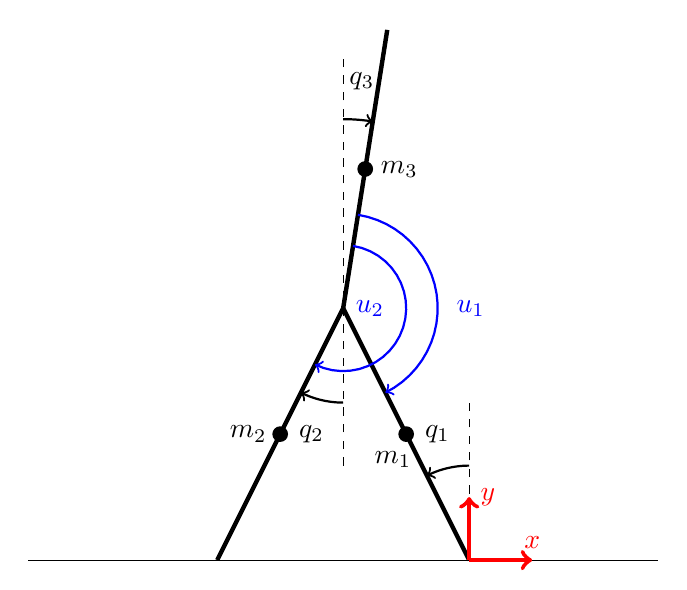
\begin{tikzpicture}
			\begin{scope}[x={8cm},y={8cm}]
				% l = 0,447213
				% alpha = 8.999999999478607 deg
				% =0.5+sqrt(0.2^2+0.4^2)*sin(pi/20)
				% =0.4+sqrt(0.2^2+0.4^2)*cos(pi/20)

				\draw[-] (0,0)--(1,0); % ground

				\draw[-,ultra thick] (0.3,0)--(0.5,0.4); % link 2
				\draw[-,ultra thick] (0.7,0)--(0.5,0.4); % link 1
				\draw[-,ultra thick] (0.5,0.4)--(0.5699596195707541,0.8417076540309386); % link 3

				\draw[dashed] (0.5,0.15)--(0.5,0.8); % big vertical dashed line
				\draw[dashed] (0.7,0)--(0.7,0.25); % small vertical dashed line

				\draw[->,ultra thick, red] (0.7,0)--(0.8,0) node[above]{$x$}; % x axis
				\draw[->,ultra thick, red] (0.7,0)--(0.7,0.1) node[right]{$y$}; % y axis

				\draw [->,thick,domain=81.00000000052139:-63.4349488, blue] plot ({0.5+0.15*cos(\x)}, {0.4+0.15*sin(\x)}); % u1
				\draw [->,thick,domain=81.00000000052139:-116.5650512, blue] plot ({0.5+0.10*cos(\x)}, {0.4+0.10*sin(\x)}); % u2

				\draw [->,thick,domain=-90:-116.5650512] plot ({0.5+0.15*cos(\x)}, {0.4+0.15*sin(\x)}); % q2
				\draw [->,thick,domain=90:116.5650512] plot ({0.7+0.15*cos(\x)}, {0.15*sin(\x)}); % q1
				\draw [->,thick,domain=90:81.00000000052139] plot ({0.5+0.3*cos(\x)}, {0.4+0.3*sin(\x)}); % q3

				\node at (0.4,0.2) [circle,fill,inner sep=1]{.}; % m2
				\node at (0.6,0.2) [circle,fill,inner sep=1]{.}; % m1
				\node at (0.5349798097853771,0.6208538270154693) [circle,fill,inner sep=1]{.}; % m3

				\node[text width=0mm] at (0.63,0.2) {$q_1$};
				\node[text width=0mm] at (0.43,0.2) {$q_2$};
				\node[text width=0mm] at (0.51,0.76) {$q_3$};

				\node[text width=0mm] at (0.55,0.16) {$m_1$};
				\node[text width=0mm] at (0.32,0.2) {$m_2$};
				\node[text width=0mm] at (0.56,0.62) {$m_3$};

				\node[text width=0mm, blue] at (0.68,0.4) {$u_1$};
				\node[text width=0mm, blue] at (0.52,0.4) {$u_2$};
			\end{scope}
		\end{tikzpicture}
	\end{center}
	\caption{Representation of the three-link 2D biped model with the angle commands.}
	\label{fig::model_with_command}
\end{figure}

This means that the model is underactuated, because there is more DOFs than actuated joints.

\vspace{\baselineskip}

The work done by $\mathbf{u}_1$ and $\mathbf{u}_2$ is computed as the product of $\mathbf{u}_i$ and the corresponding virtual angle variation.
Then, the control matrix is computed by substitution.

\vspace{\baselineskip}

The obtained matrices are:

\begin{align*}
	\mathbf{M} &= \begin{bmatrix}
		{l_{1}}^2\,\left(\dfrac{m_{1}}{4}+m_{2}+m_{3}\right) & -\dfrac{l_{1}\,l_{2}\,m_{2}\,\cos\left(q_{1}-q_{2}\right)}{2} & \dfrac{l_{1}\,l_{3}\,m_{3}\,\cos\left(q_{1}-q_{3}\right)}{2}\\ -\dfrac{l_{1}\,l_{2}\,m_{2}\,\cos\left(q_{1}-q_{2}\right)}{2} & \dfrac{{l_{2}}^2\,m_{2}}{4} & 0\\ \dfrac{l_{1}\,l_{3}\,m_{3}\,\cos\left(q_{1}-q_{3}\right)}{2} & 0 & \dfrac{{l_{3}}^2\,m_{3}}{4}
	\end{bmatrix} \\
	\mathbf{C} &= \begin{bmatrix}
		0 & -\dfrac{\mathrm{dq}_{2}\,l_{1}\,l_{2}\,m_{2}\,\sin\left(q_{1}-q_{2}\right)}{2} & \dfrac{\mathrm{dq}_{3}\,l_{1}\,l_{3}\,m_{3}\,\sin\left(q_{1}-q_{3}\right)}{2}\\ \dfrac{\mathrm{dq}_{1}\,l_{1}\,l_{2}\,m_{2}\,\sin\left(q_{1}-q_{2}\right)}{2} & 0 & 0\\ -\dfrac{\mathrm{dq}_{1}\,l_{1}\,l_{3}\,m_{3}\,\sin\left(q_{1}-q_{3}\right)}{2} & 0 & 0
	\end{bmatrix} \\
	\mathbf{G} &= \begin{bmatrix}
		-\dfrac{g\,l_{1}\,\sin\left(q_{1}\right)\,\left(m_{1}+2\,m_{2}+2\,m_{3}\right)}{2}\\ \dfrac{g\,l_{2}\,m_{2}\,\sin\left(q_{2}\right)}{2}\\ -\dfrac{g\,l_{3}\,m_{3}\,\sin\left(q_{3}\right)}{2}
	\end{bmatrix} \\
	\mathbf{B} &= \begin{bmatrix}
		1 & 0\\ 0 & 1\\ -1 & -1
	\end{bmatrix}
\end{align*}

It is interesting to notice that the mass matrix $\mathbf{M}$ corresponds to the Jacobian of the total kinetic energy $T$ with respect to the generalized coordinates.
That is a normal result, since kinetic energy is derived from moving masses.% (\textbf{assignement 1 question}).

\subsubsection{Impact map}

% generate impact map.mlx (in the “generate model” folder)
% eval A m.m, eval A p.m (in the “dynamics” folder)
% impact.m (in the “dynamics” folder)

In the hybrid model of walking, the model oscillates between the single support swing phase and the impact phase, during which the leg roles are switched, like so:

\begin{center}
	\begin{tikzpicture}[auto]
		\node [block] (swing) {Single support swing phase};
		\node [block, right=of swing] (impact) {Impact phase};

		\draw [->] (swing) |- (0, 1.5) -| (impact);
		\draw [<-] (swing) |- (0, -1.5) -| (impact);
	\end{tikzpicture}
\end{center}

The modelization of the swing phase has been extensively described in the previous sections, leading to the kinematics and dynamics of the robot during the single support swing phase through the Lagrangian method.

\vspace{\baselineskip}

This section is concerned with the impact phase.
This phase is based on the assumptions that:

\begin{itemize}
	\item the impact and leg role switching is instantaneous and
	\item the support leg does not slip.
\end{itemize}

Because of the assumption of instantaneousness, there is no need for (and it would prove to be quite difficult to) develop kinematics and dynamics for the impact phase.
Instead, the state of the robot is mapped from right before the impact to right after the impact, throught the use of the impact map $\mathbf{\Delta}$ computed by conservation of the angular momentum.
In particular, we can write:

\begin{align*}
	\mathbf{\Delta} \left( \mathbf{q}_m, \mathbf{\dot{q}}_m \right) &= \begin{bmatrix}
		\mathbf{\Delta}_q \left( \mathbf{q}_m \right) &  \mathbf{\Delta}_{\dot{q}} \left( \mathbf{q}_m, \mathbf{\dot{q}}_m \right)
	\end{bmatrix}
\end{align*}

The angular positions are the same (semantically) before and after impact, so the mapping only needs to account for the change of reference frame.

\vspace{\baselineskip}

On the contrary, the angular velocities after impact are computed using the McGeer method~\cite{mcgeer}, which is a conservation of angular momentum method: the angular momentum before impact $H_m$ must be equal to the angular momentum after impact $H_p$:

\begin{align*}
	H_m &= H_p \\
	A_m\mathbf{\dot{q}}_m &= A_p\mathbf{\dot{q}}_p \\
	\mathbf{\dot{q}}_p &= A_{p}^{-1}A_m\mathbf{\dot{q}}_m
\end{align*}

After computation:

\tiny

\begin{align*}
	A_p &= \begin{bmatrix}
		\dfrac{l_{1}\,l_{2}\,m\,\cos\left(q_{1,p}-q_{2,p}\right)}{2}-{l_{1}}^2\,m_{3}-\dfrac{5\,{l_{1}}^2\,m}{4}-\dfrac{l_{1}\,l_{3}\,m_{3}\,\cos\left(q_{1,p}-q_{3,p}\right)}{2} & \dfrac{l_{1}\,l_{2}\,m\,\cos\left(q_{1,p}-q_{2,p}\right)}{2}-\dfrac{{l_{2}}^2\,m}{4} & -\dfrac{m_{3}\,{l_{3}}^2}{4}-\dfrac{l_{1}\,m_{3}\,\cos\left(q_{1,p}-q_{3,p}\right)\,l_{3}}{2}\\ \dfrac{l_{1}\,l_{2}\,m_{3}\,\cos\left(q_{1,p}-q_{2,p}\right)}{2} & -\dfrac{{l_{2}}^2\,m_{3}}{4} & 0\\ -\dfrac{l_{1}\,l_{3}\,m\,\cos\left(q_{1,p}-q_{3,p}\right)}{2} & 0 & -\dfrac{{l_{3}}^2\,m}{4}
	\end{bmatrix} \\
	A_m &= \begin{bmatrix}
		\dfrac{{l_{1}}^2\,m}{4}-l_{1}\,l_{2}\,m\,\cos\left(q_{1,m}-q_{2,m}\right)-l_{1}\,l_{2}\,m_{3}\,\cos\left(q_{1,m}-q_{2,m}\right)-\dfrac{l_{1}\,l_{3}\,m_{3}\,\cos\left(q_{1,m}-q_{3,m}\right)}{2} & \dfrac{{l_{2}}^2\,m}{4} & -\dfrac{m_{3}\,{l_{3}}^2}{4}-\dfrac{l_{2}\,m_{3}\,\cos\left(q_{2,m}-q_{3,m}\right)\,l_{3}}{2}\\ \dfrac{{l_{1}}^2\,m_{3}}{4} & 0 & 0\\ -\dfrac{l_{1}\,l_{3}\,m\,\cos\left(q_{1,m}-q_{3,m}\right)}{2} & 0 & -\dfrac{{l_{3}}^2\,m}{4}
	\end{bmatrix}
\end{align*}

\normalsize

with $m=m_1=m_2$, and thus both $\mathbf{q}_p$ and $\mathbf{\dot{q}}_p$ can be computed.

\vspace{\baselineskip}

\textbf{Assignement 2 questions:}

\begin{enumerate}
	\item \textit{What can you say about the potential energy before and after impact?}
	
	The potential energy before and after the impact are the same, since the frame of reference is moved from one foot to another without any change in the position, velocity or acceleration of the different masses.
	\item \textit{Try $\mathbf{q}_m = \begin{bmatrix}
		pi/6 & -pi/6 & pi/10
	\end{bmatrix}$, $\mathbf{\dot{q}}_m = \begin{bmatrix}
		1 & 0.2 & 0
	\end{bmatrix}$. What percentage of the kinetic energy of the biped is lost due to the impact?}

	Computing using our functions, we find that 38.73\% of the kinetic energy is lost during the impact of the foot for those parameters.
	\item \textit{Plot the percentage of the kinetic energy loss due to impact as a function of angle $\alpha$ where $\mathbf{q}_m=\begin{bmatrix}
		\alpha & -\alpha & 0
	\end{bmatrix}$ and $\alpha$ varies from 0 to $\pi/4$. Assume that $\mathbf{\dot{q}} = \begin{bmatrix}
		1 & 0.2 & 0
	\end{bmatrix}$.}

	\begin{figure}[H]
		\begin{center}
			\includegraphics[angle=0,width=0.7\textwidth]{kinetic_energy_loss_along_leg_angle}
		\end{center}
		\caption{Percentage of kinetic energy loss as a function of leg angle.}
	\end{figure}
	\item \textit{The bigger $\alpha$ is, the bigger is the step length. Based on your answer to question 3, what is the relation between step length and energy loss at impact given a fixed $\mathbf{\dot{q}}_m$?}
	
	The energy loss appears to be akin to a square root function. The bigger the step, the bigger the energy loss : if there is no step at all (i.e. if $\alpha=0$), there is no energy loss. If we were to optimize the energy loss over the distance travelled, we'd have to look for the inflexion point (which is approximately at $\alpha = \SI{0.15}{\radian}$), because the energy loss increases slowlier at first (from $\alpha=0$ to $\alpha\sim\SI{0.15}{\radian}$), and then faster.  
\end{enumerate}
